\documentclass[10pt]{article}
\usepackage[margin=1in]{geometry}
\usepackage[T1]{fontenc}
\usepackage{lmodern,microtype,booktabs,graphicx,xcolor,amsmath,amssymb}
\usepackage[numbers,sort&compress]{natbib}
\usepackage[colorlinks=true,linkcolor=blue!50!black,citecolor=blue!50!black,urlcolor=blue!50!black]{hyperref}
\usepackage{tikz}
\usetikzlibrary{positioning,arrows.meta,fit,backgrounds}
\usepackage{caption}
\captionsetup{font=small,labelfont=bf}
\newcommand{\routeridtask}{99.6}
\newcommand{\routeridepisode}{97.4}
\newcommand{\routeridquick}{98.4}
\newcommand{\routeridcancel}{100.0}
\newcommand{\routeridrevise}{100.0}
\newcommand{\routeridquicklat}{7}
\newcommand{\routeridtokens}{294}
\newcommand{\oraclerouteridtask}{99.5}
\newcommand{\oraclerouteridepisode}{97.0}
\newcommand{\oraclerouteridquick}{98.2}
\newcommand{\oraclerouteridcancel}{99.3}
\newcommand{\oraclerouteridrevise}{100.0}
\newcommand{\oraclerouteridquicklat}{7}
\newcommand{\oraclerouteridtokens}{293}
\newcommand{\tagsidtask}{99.4}
\newcommand{\tagsidepisode}{96.4}
\newcommand{\tagsidquick}{98.2}
\newcommand{\tagsidcancel}{99.3}
\newcommand{\tagsidrevise}{99.7}
\newcommand{\tagsidquicklat}{9}
\newcommand{\tagsidtokens}{320}
\newcommand{\oracletagsidtask}{99.6}
\newcommand{\oracletagsidepisode}{97.7}
\newcommand{\oracletagsidquick}{98.7}
\newcommand{\oracletagsidcancel}{99.3}
\newcommand{\oracletagsidrevise}{100.0}
\newcommand{\oracletagsidquicklat}{9}
\newcommand{\oracletagsidtokens}{318}
\newcommand{\orchidtask}{97.6}
\newcommand{\orchidepisode}{87.1}
\newcommand{\orchidquick}{91.5}
\newcommand{\orchidcancel}{100.0}
\newcommand{\orchidrevise}{100.0}
\newcommand{\orchidquicklat}{11}
\newcommand{\orchidtokens}{359}
\newcommand{\oracleorchidtask}{97.5}
\newcommand{\oracleorchidepisode}{86.7}
\newcommand{\oracleorchidquick}{91.2}
\newcommand{\oracleorchidcancel}{100.0}
\newcommand{\oracleorchidrevise}{100.0}
\newcommand{\oracleorchidquicklat}{11}
\newcommand{\oracleorchidtokens}{361}
\newcommand{\turnidtask}{66.5}
\newcommand{\turnidepisode}{4.3}
\newcommand{\turnidquick}{11.7}
\newcommand{\turnidcancel}{1.4}
\newcommand{\turnidrevise}{99.7}
\newcommand{\turnidquicklat}{206}
\newcommand{\turnidtokens}{338}
\newcommand{\oracleturnidtask}{66.4}
\newcommand{\oracleturnidepisode}{4.3}
\newcommand{\oracleturnidquick}{11.7}
\newcommand{\oracleturnidcancel}{0.7}
\newcommand{\oracleturnidrevise}{100.0}
\newcommand{\oracleturnidquicklat}{207}
\newcommand{\oracleturnidtokens}{338}
\newcommand{\routerstresstask}{97.7}
\newcommand{\routerstressepisode}{81.8}
\newcommand{\routerstressquick}{99.4}
\newcommand{\routerstresscancel}{96.8}
\newcommand{\routerstressrevise}{95.2}
\newcommand{\routerstressquicklat}{7}
\newcommand{\routerstresstokens}{515}
\newcommand{\oraclerouterstresstask}{99.9}
\newcommand{\oraclerouterstressepisode}{99.3}
\newcommand{\oraclerouterstressquick}{99.8}
\newcommand{\oraclerouterstresscancel}{99.7}
\newcommand{\oraclerouterstressrevise}{100.0}
\newcommand{\oraclerouterstressquicklat}{7}
\newcommand{\oraclerouterstresstokens}{513}
\newcommand{\tagsstresstask}{96.8}
\newcommand{\tagsstressepisode}{77.0}
\newcommand{\tagsstressquick}{99.6}
\newcommand{\tagsstresscancel}{97.2}
\newcommand{\tagsstressrevise}{93.7}
\newcommand{\tagsstressquicklat}{9}
\newcommand{\tagsstresstokens}{546}
\newcommand{\oracletagsstresstask}{99.9}
\newcommand{\oracletagsstressepisode}{99.3}
\newcommand{\oracletagsstressquick}{99.8}
\newcommand{\oracletagsstresscancel}{100.0}
\newcommand{\oracletagsstressrevise}{100.0}
\newcommand{\oracletagsstressquicklat}{9}
\newcommand{\oracletagsstresstokens}{556}
\newcommand{\orchstresstask}{98.0}
\newcommand{\orchstressepisode}{85.8}
\newcommand{\orchstressquick}{98.1}
\newcommand{\orchstresscancel}{97.8}
\newcommand{\orchstressrevise}{98.0}
\newcommand{\orchstressquicklat}{8}
\newcommand{\orchstresstokens}{628}
\newcommand{\oracleorchstresstask}{99.5}
\newcommand{\oracleorchstressepisode}{96.0}
\newcommand{\oracleorchstressquick}{98.2}
\newcommand{\oracleorchstresscancel}{100.0}
\newcommand{\oracleorchstressrevise}{100.0}
\newcommand{\oracleorchstressquicklat}{8}
\newcommand{\oracleorchstresstokens}{619}
\newcommand{\turnstresstask}{60.3}
\newcommand{\turnstressepisode}{0.0}
\newcommand{\turnstressquick}{6.3}
\newcommand{\turnstresscancel}{0.0}
\newcommand{\turnstressrevise}{100.0}
\newcommand{\turnstressquicklat}{487}
\newcommand{\turnstresstokens}{660}
\newcommand{\oracleturnstresstask}{60.3}
\newcommand{\oracleturnstressepisode}{0.0}
\newcommand{\oracleturnstressquick}{6.3}
\newcommand{\oracleturnstresscancel}{0.0}
\newcommand{\oracleturnstressrevise}{100.0}
\newcommand{\oracleturnstressquicklat}{487}
\newcommand{\oracleturnstresstokens}{659}
\newcommand{\dtagsidtask}{+0.2}
\newcommand{\dtagsidtaskci}{[-0.2, +0.5]}
\newcommand{\dtagsidepisode}{+1.0}
\newcommand{\dtagsidepisodeci}{[-1.1, +3.0]}
\newcommand{\dtagsidquick}{+0.2}
\newcommand{\dtagsidquickci}{[-1.2, +1.6]}
\newcommand{\dtagsidquicklat}{-1.3}
\newcommand{\dtagsidquicklatci}{[-1.7, -0.8]}
\newcommand{\dtagsidtokens}{-25.3}
\newcommand{\dtagsidtokensci}{[-27.2, -23.7]}
\newcommand{\dorchidtask}{+2.0}
\newcommand{\dorchidtaskci}{[+1.3, +2.7]}
\newcommand{\dorchidepisode}{+10.3}
\newcommand{\dorchidepisodeci}{[+6.8, +14.2]}
\newcommand{\dorchidquick}{+6.9}
\newcommand{\dorchidquickci}{[+4.3, +9.8]}
\newcommand{\dorchidquicklat}{-3.6}
\newcommand{\dorchidquicklatci}{[-4.3, -2.9]}
\newcommand{\dorchidtokens}{-65.1}
\newcommand{\dorchidtokensci}{[-69.7, -60.7]}
\newcommand{\dturnidtask}{+33.1}
\newcommand{\dturnidtaskci}{[+31.5, +34.8]}
\newcommand{\dturnidepisode}{+93.1}
\newcommand{\dturnidepisodeci}{[+90.3, +95.6]}
\newcommand{\dturnidquick}{+86.7}
\newcommand{\dturnidquickci}{[+83.3, +89.9]}
\newcommand{\dturnidquicklat}{-199.2}
\newcommand{\dturnidquicklatci}{[-212.5, -185.8]}
\newcommand{\dturnidtokens}{-43.7}
\newcommand{\dturnidtokensci}{[-47.6, -40.0]}
\newcommand{\drouternoembidtask}{+0.1}
\newcommand{\drouternoembidtaskci}{[-0.1, +0.2]}
\newcommand{\drouternoembidepisode}{+0.4}
\newcommand{\drouternoembidepisodeci}{[-0.7, +1.4]}
\newcommand{\drouternoembidquick}{-0.1}
\newcommand{\drouternoembidquickci}{[-0.6, +0.4]}
\newcommand{\drouternoembidquicklat}{+0.0}
\newcommand{\drouternoembidquicklatci}{[-0.1, +0.2]}
\newcommand{\drouternoembidtokens}{+0.1}
\newcommand{\drouternoembidtokensci}{[-0.2, +0.5]}
\newcommand{\dtagsstresstask}{+0.9}
\newcommand{\dtagsstresstaskci}{[+0.5, +1.4]}
\newcommand{\dtagsstressepisode}{+4.8}
\newcommand{\dtagsstressepisodeci}{[+1.6, +7.9]}
\newcommand{\dtagsstressquick}{-0.2}
\newcommand{\dtagsstressquickci}{[-0.8, +0.4]}
\newcommand{\dtagsstressquicklat}{-1.6}
\newcommand{\dtagsstressquicklatci}{[-1.7, -1.4]}
\newcommand{\dtagsstresstokens}{-31.2}
\newcommand{\dtagsstresstokensci}{[-39.5, -20.6]}
\newcommand{\dorchstresstask}{-0.3}
\newcommand{\dorchstresstaskci}{[-0.8, +0.1]}
\newcommand{\dorchstressepisode}{-4.0}
\newcommand{\dorchstressepisodeci}{[-7.3, -0.8]}
\newcommand{\dorchstressquick}{+1.3}
\newcommand{\dorchstressquickci}{[+0.3, +2.3]}
\newcommand{\dorchstressquicklat}{-1.4}
\newcommand{\dorchstressquicklatci}{[-1.7, -1.1]}
\newcommand{\dorchstresstokens}{-113.3}
\newcommand{\dorchstresstokensci}{[-129.2, -99.3]}
\newcommand{\dturnstresstask}{+37.4}
\newcommand{\dturnstresstaskci}{[+36.5, +38.3]}
\newcommand{\dturnstressepisode}{+81.8}
\newcommand{\dturnstressepisodeci}{[+78.2, +84.9]}
\newcommand{\dturnstressquick}{+93.1}
\newcommand{\dturnstressquickci}{[+90.9, +95.1]}
\newcommand{\dturnstressquicklat}{-479.8}
\newcommand{\dturnstressquicklatci}{[-504.7, -453.9]}
\newcommand{\dturnstresstokens}{-145.0}
\newcommand{\dturnstresstokensci}{[-153.3, -134.4]}
\newcommand{\drouternoembstresstask}{+0.2}
\newcommand{\drouternoembstresstaskci}{[-0.2, +0.6]}
\newcommand{\drouternoembstressepisode}{-0.6}
\newcommand{\drouternoembstressepisodeci}{[-3.2, +2.1]}
\newcommand{\drouternoembstressquick}{+0.1}
\newcommand{\drouternoembstressquickci}{[-0.3, +0.5]}
\newcommand{\drouternoembstressquicklat}{-0.0}
\newcommand{\drouternoembstressquicklatci}{[-0.1, +0.0]}
\newcommand{\drouternoembstresstokens}{-12.1}
\newcommand{\drouternoembstresstokensci}{[-27.1, +2.7]}
\newcommand{\longrouterfulltask}{84.3}
\newcommand{\longrouterfullepisode}{20.8}
\newcommand{\longrouterfullrevise}{78.5}
\newcommand{\longrouterfullcancel}{74.9}
\newcommand{\longrouterfullplain}{87.3}
\newcommand{\longrouterfulltokens}{4578}
\newcommand{\longroutermemtask}{97.8}
\newcommand{\longroutermemepisode}{50.0}
\newcommand{\longroutermemrevise}{97.3}
\newcommand{\longroutermemcancel}{96.1}
\newcommand{\longroutermemplain}{98.1}
\newcommand{\longroutermemtokens}{2481}
\newcommand{\longrouterplaintask}{97.7}
\newcommand{\longrouterplainepisode}{49.0}
\newcommand{\longrouterplainrevise}{97.9}
\newcommand{\longrouterplaincancel}{96.0}
\newcommand{\longrouterplainplain}{98.1}
\newcommand{\longrouterplaintokens}{2506}
\newcommand{\longtagsfulltask}{91.9}
\newcommand{\longtagsfullepisode}{14.6}
\newcommand{\longtagsfullrevise}{93.4}
\newcommand{\longtagsfullcancel}{95.9}
\newcommand{\longtagsfullplain}{90.0}
\newcommand{\longtagsfulltokens}{2910}
\newcommand{\longtagsmemtask}{95.0}
\newcommand{\longtagsmemepisode}{44.8}
\newcommand{\longtagsmemrevise}{94.6}
\newcommand{\longtagsmemcancel}{97.3}
\newcommand{\longtagsmemplain}{94.2}
\newcommand{\longtagsmemtokens}{2853}
\newcommand{\longtagsplaintask}{96.3}
\newcommand{\longtagsplainepisode}{53.1}
\newcommand{\longtagsplainrevise}{96.2}
\newcommand{\longtagsplaincancel}{97.7}
\newcommand{\longtagsplainplain}{96.2}
\newcommand{\longtagsplaintokens}{2792}
\newcommand{\dlongroutertask}{+0.1}
\newcommand{\dlongroutertaskci}{[-0.6, +0.7]}
\newcommand{\dlongroutertaskp}{0.756}
\newcommand{\dlongrouterrevise}{-0.6}
\newcommand{\dlongrouterreviseci}{[-1.7, +0.0]}
\newcommand{\dlongrouterrevisep}{0.269}
\newcommand{\dlongroutercancel}{+0.2}
\newcommand{\dlongroutercancelci}{[-0.6, +0.8]}
\newcommand{\dlongroutercancelp}{0.764}
\newcommand{\dlongrouterepisode}{+1.0}
\newcommand{\dlongrouterepisodeci}{[-5.2, +7.3]}
\newcommand{\dlongrouterepisodep}{0.836}
\newcommand{\dlongtagstask}{-1.3}
\newcommand{\dlongtagstaskci}{[-2.5, -0.4]}
\newcommand{\dlongtagstaskp}{0.002}
\newcommand{\dlongtagsrevise}{-1.5}
\newcommand{\dlongtagsreviseci}{[-4.2, +0.9]}
\newcommand{\dlongtagsrevisep}{0.236}
\newcommand{\dlongtagscancel}{-0.4}
\newcommand{\dlongtagscancelci}{[-2.5, +1.4]}
\newcommand{\dlongtagscancelp}{0.691}
\newcommand{\dlongtagsepisode}{-8.3}
\newcommand{\dlongtagsepisodeci}{[-17.7, +0.0]}
\newcommand{\dlongtagsepisodep}{0.079}
\newcommand{\gsmbase}{38.3}
\newcommand{\gsmbasethink}{53.7}
\newcommand{\gsmsolo}{52.0}
\newcommand{\gsmsolonoalign}{49.7}
\newcommand{\gsmasync}{45.7}
\newcommand{\gsmasyncnoalign}{46.3}
\newcommand{\gsmasyncquick}{97.3}
\newcommand{\gsmasyncquicknoalign}{96.5}
\newcommand{\visall}{95.3}
\newcommand{\visallnoalign}{42.2}
\newcommand{\viscountcolor}{94.0}
\newcommand{\viscountcolornoalign}{42.7}
\newcommand{\viscountshape}{88.8}
\newcommand{\viscountshapenoalign}{32.9}
\newcommand{\visexists}{98.7}
\newcommand{\visexistsnoalign}{69.6}
\newcommand{\viscolorof}{100.0}
\newcommand{\viscolorofnoalign}{20.7}
\newcommand{\visother}{99.6}
\newcommand{\visothernoalign}{99.3}
\newcommand{\mmidtask}{99.8}
\newcommand{\mmidtasknoalign}{99.7}
\newcommand{\gsmdiff}{-6.3}
\newcommand{\gsmdiffci}{[-10.7, -2.0]}
\newcommand{\gsmdiffnoalign}{-3.3}
\newcommand{\gsmdiffcinoalign}{[-7.7, +1.0]}
\newcommand{\gsmthinktrunc}{22}
\newcommand{\gsmvsthink}{-1.7}
\newcommand{\gsmvsthinkci}{[-8.0, +5.0]}
\newcommand{\gsmthinkclause}{ and 53.7\% in its built-in thinking mode (up to 1536 generated tokens; 22\% of outputs without a parseable answer)}
\newcommand{\gsmthinktok}{116}

\providecommand{\gsmthinkclause}{}
\providecommand{\TODO}{\textbf{??}}

\title{An Always-On Language Model with a Learned Output Router:\\
Routing Thought, Speech, Writing, Code and Action from a Single Stream}
\author{Siavash Shirzadeh Barough\\\small Preprint}
\date{\small October 2026}

\begin{document}
\maketitle

\begin{abstract}
Large language models (LLMs) are usually run as turn-based generators that stop at an end-of-sequence (EOS) token and are wrapped in external agent loops that decide when to think, speak, call a tool, or wait. We propose and test a simpler organisation, inspired by the functional layout of the brain, in which sensory inputs, an ongoing stream of thought and several executive outputs share one continuous workspace, and a selection mechanism decides, token by token, which output a computation drives. A decoder-only LLM emits a single token stream; a small learned \emph{router head} assigns every generated token to one of seven channels (think, say, write, code, exec, mem, idle); EOS is replaced by an \emph{idle} channel, so the model never terminates and waits for the next event; external events (user messages, tool results, images) are inserted into the stream at the time they arrive, including mid-thought; and tokens routed to a \emph{mem} channel are retained when old context is evicted. We fine-tuned Qwen3-0.6B by imitation of scripted policies in AsyncWorld, a synthetic environment with concurrent tasks, deadlines, cancellations, revisions and asynchronous tools, and compared the router with three control protocols trained on identical episodes: in-stream channel tags, a rule-based orchestrator that delivers events only at line boundaries, and a turn-based agent loop (3 seeds per arm, 300 test episodes per split). The router matched tags in distribution (task success \routeridtask\% vs.\ \tagsidtask\%) and was slightly more accurate on a heavier, out-of-distribution load (\dtagsstresstask\,pp, 95\% CI \dtagsstresstaskci\ over episodes; smaller than the seed-to-seed spread), while saving the tokens that tags spend on channel switches. Compared with the orchestrator, it answered deadline-bound requests more often in distribution (\dorchidquick\,pp) with fewer tokens, but under the heavier load overall task success was similar and whole-episode success was lower (\dorchstressepisode\,pp, CI \dorchstressepisodeci). The turn-based loop, which by construction cannot respond while blocked, met few deadlines (\turnidquick\% vs.\ \routeridquick\%). In a multimodal pilot with a frozen CLIP-ConvNeXt image encoder and self-distilled GSM8K rationales routed to the think channel, one router model answered \visall\% of visual questions on held-out synthetic scenes and solved \gsmsolo\% of GSM8K problems, comparable to the base model's built-in thinking mode (\gsmbasethink\%); urgent requests arriving mid-thought were answered on time (\gsmasyncquick\%) but reduced math accuracy by \gsmdiff\,pp (CI \gsmdiffci). Retaining mem-routed tokens did not change long-horizon success, as the environment rarely required information older than the recent context window. These small-scale, synthetic results show that output routing, waiting and interruption handling can be learned inside the model rather than hard-coded around it; they do not show benefits on natural tasks or at scale.
\end{abstract}

\section{Introduction}
A human does not alternate between a ``thinking program'' and a ``speaking program'' orchestrated from outside. Perception, ongoing thought and action run concurrently, and a person can stop mid-thought to answer a question, resume, wait, or remember to finish a task later. Current LLM agents obtain similar behaviour through scaffolding: the model generates until EOS, and an external controller parses the output, routes it to tools or the user, decides when the model may continue, and re-prompts it with new observations \citep{yao2022react,schick2023toolformer,packer2023memgpt}. This scaffolding is hand-written, turn-based, and blind to the model's internal state, so the model cannot be interrupted between turns and cannot keep thinking while it waits.

We ask whether this control can be moved inside the model with minimal machinery. Our proposal has four components:
\begin{enumerate}\itemsep0pt
\item \textbf{One stream, many outputs.} The model emits one token per tick. A linear router head on the final hidden state predicts the output channel of each token (think, say, write, code, exec, mem, idle). Channel identity is fed back through a learned channel embedding, so the model knows which ``effector'' produced each past token.
\item \textbf{No stop token.} EOS is removed from the action space and replaced by an \emph{idle} channel. Idle advances the clock to the next event; the model never terminates.
\item \textbf{Event-timed inputs.} User messages, tool results and images are inserted into the stream at the tick at which they arrive, even in the middle of a line of thought, and training sequences contain such insertions, so the model learns to react to them without an external controller.
\item \textbf{Memory by routing.} Tokens routed to the mem channel are retained when old context is evicted, giving a learned, content-addressed retention policy under a fixed context budget.
\end{enumerate}

The design is motivated by a coarse functional analogy to the brain (Section~\ref{sec:brain}): a shared workspace that broadcasts to many specialised processors \citep{baars1988cognitive,dehaene1998neuronal}, a selection system that gates one action among competing ones \citep{mink1996basal,redgrave1999basal}, intrinsic activity that persists without external input \citep{raichle2001default}, and a separate system for retaining selected episodes \citep{mcclelland1995why}. We use the analogy to generate design hypotheses, not as a claim of biological fidelity.

Throughout, time is measured in \emph{ticks}: one generated token takes one tick, inserted input tokens take none, and waiting (idle) advances the clock to the next event; latency is the number of ticks between a request's arrival and its answer. Training data come from an \emph{oracle}, a hand-written scripted policy for each control protocol, whose own score gives an upper reference (``oracle ceiling'') for a model that imitates it.

\paragraph{Contributions.} (i) An architecture and training recipe for an always-on LLM with a learned per-token output router, an idle channel in place of EOS, event-timed input insertion, and mem-routed retention. (ii) AsyncWorld, a controlled benchmark with concurrent tasks, deadlines, cancellations, revisions and asynchronous tools, together with scripted oracle policies for four control protocols. (iii) A comparison with hypotheses specified before the main runs against in-stream tags, a rule-based orchestrator and a turn-based loop at equal data, with three seeds per arm and paired bootstrap CIs. (iv) A multimodal pilot in which vision and step-by-step math reasoning share the same routed stream.

\section{Related work}\label{sec:related}
\paragraph{Continuous and asynchronous LLM agents.} The closest work trains a single think/say/tool stream for continuous-time agents, but an external orchestrator of about 200 lines ``alone knows the clock'', forces the end of thoughts, and injects events at interrupt points as chat turns \citep{li2026never}. Multi-Stream LLMs decode several role-fixed streams in lockstep with per-stream positions and stream embeddings; streams are fixed rather than learned \citep{su2026multistream}. Asynchronous Reasoning lets a thinker and a writer share one KV cache, with the writer gated by an inserted probe every paragraph, training-free \citep{yakushev2025asynchronous}. Asynchronous function calling \citep{gim2024asynclm,shi2026asynctool} and interruptibility benchmarks \citep{wu2025interruptible,zou2026users} study how agents handle tools and users that change their minds. Parallel decoding methods (Hogwild!, Multiverse) run several reasoning threads concurrently \citep{rodionov2025hogwild,yang2025multiverse}. Our design differs in that channel selection is a learned per-token decision on one stream, termination is replaced by a learned idle action, and inputs are inserted at their arrival tick without a controller.

\paragraph{Full-duplex dialogue.} Spoken dialogue models listen and speak simultaneously \citep{defossez2024moshi,veluri2024syncllm,ma2024lslm,zhang2024beyond}, and SHANKS lets a spoken model think while listening \citep{chiang2025shanks}. A recent duplex agent uses a learned per-second control token (listen/speak/interrupt) and delegates tasks to a separate agent \citep{orantqing2026gander}. These systems route between at most a few speech states at a coarse time step; we route every token among seven text-level channels including thought, code and memory.

\paragraph{Latent and hidden reasoning.} Pause tokens \citep{goyal2023pause}, Quiet-STaR \citep{zelikman2024quietstar} and continuous latent reasoning \citep{hao2024coconut} separate internal computation from output. STaR bootstraps rationales from a model's own correct answers \citep{zelikman2022star}; we use the same idea to obtain think-channel content.

\paragraph{Workspace models in deep learning.} Global-workspace ideas have been proposed for deep networks \citep{vanrullen2021deep} and implemented as a shared bottleneck among neural modules \citep{goyal2021coordination}. Our model uses a pretrained LLM as the shared workspace and adds a router as the selection mechanism.

\paragraph{Memory.} MemGPT manages memory through explicit function calls issued by the model and executed by a controller \citep{packer2023memgpt}. Our mem channel is an output like any other; retention is a side effect of routing.

\section{A brain-inspired organisation}\label{sec:brain}
Figure~\ref{fig:arch} and Table~\ref{tab:brain} summarise the analogy that guided the design. We list the neuroscience findings that motivated each component and state explicitly what we did and did not implement. The analogy is functional and coarse; we do not claim that the network computes as the brain does.

\begin{figure}[t]
\centering
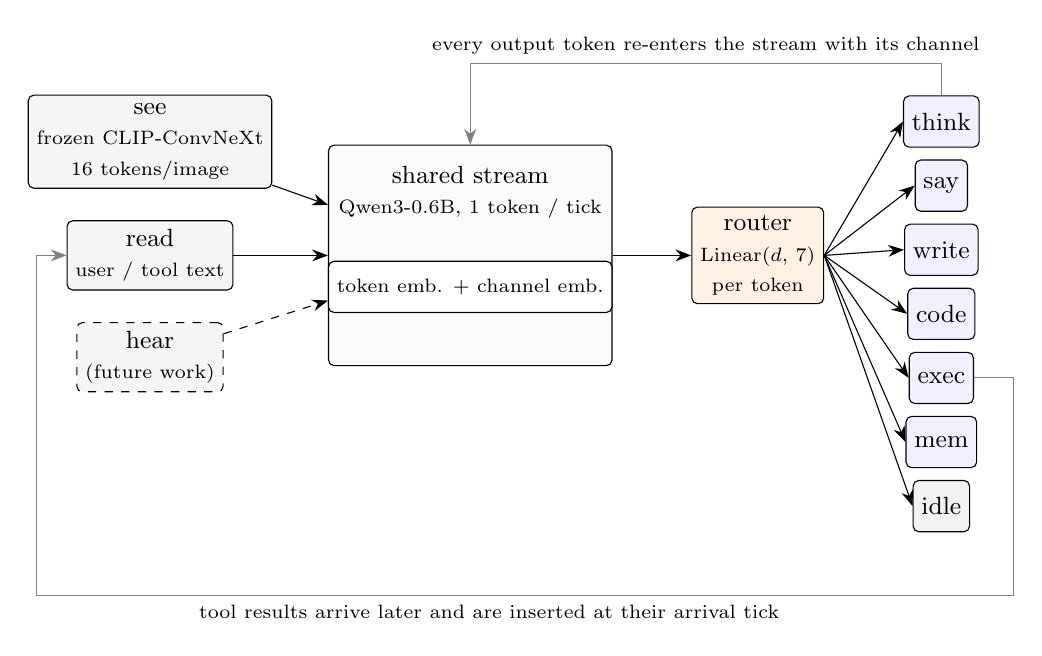
\begin{tikzpicture}[font=\small, node distance=4mm and 6mm,
  box/.style={draw, rounded corners=2pt, minimum height=6.5mm, inner sep=3pt, align=center},
  sense/.style={box, fill=gray!8}, chan/.style={box, fill=blue!6}, ar/.style={-{Stealth[length=2mm]}}]
\node[sense] (see) {see\\\scriptsize frozen CLIP-ConvNeXt\\\scriptsize 16 tokens/image};
\node[sense, below=of see] (read) {read\\\scriptsize user / tool text};
\node[sense, below=of read, dashed] (hear) {hear\\\scriptsize (future work)};
\node[box, right=12mm of read, minimum width=36mm, minimum height=28mm, fill=gray!3] (ws) {};
\node[align=center, font=\small] at ([yshift=8mm]ws.center) {shared stream\\\scriptsize Qwen3-0.6B, 1 token / tick};
\node[box, fill=white] at ([yshift=-4mm]ws.center) (emb) {\scriptsize token emb. + channel emb.};
\node[box, right=10mm of ws, fill=orange!10] (router) {router\\\scriptsize Linear($d$, 7)\\\scriptsize per token};
\node[chan, right=10mm of router, yshift=17mm] (think) {think};
\node[chan, below=1.5mm of think] (say) {say};
\node[chan, below=1.5mm of say] (write) {write};
\node[chan, below=1.5mm of write] (code) {code};
\node[chan, below=1.5mm of code] (exec) {exec};
\node[chan, below=1.5mm of exec] (mem) {mem};
\node[chan, below=1.5mm of mem, fill=gray!10] (idle) {idle};
\draw[ar] (see) -- (ws); \draw[ar] (read) -- (ws); \draw[ar, dashed] (hear) -- (ws);
\draw[ar] (ws) -- (router);
\foreach \n in {think,say,write,code,exec,mem,idle} \draw[ar] (router.east) -- (\n.west);
\draw[ar, gray] (think.north) -- ++(0,4mm) -| node[pos=0.25, above, font=\scriptsize, text=black] {every output token re-enters the stream with its channel} (ws.north);
\draw[ar, gray] (exec.east) -- ++(5mm,0) |- ([yshift=-8mm]idle.south) -| node[pos=0.25, below, font=\scriptsize, text=black]{tool results arrive later and are inserted at their arrival tick} ([xshift=-5mm]hear.west) |- (read.west);
\end{tikzpicture}
\caption{Architecture. Senses write tokens into one stream; the router assigns each generated token to an output channel; all tokens, including inputs inserted mid-thought, are fed back with a channel embedding. There is no stop token: idle waits for the next event, and mem-routed tokens are kept when old context is evicted.}
\label{fig:arch}
\end{figure}

\begin{table}[t]
\centering\small
\caption{Functional analogy used as a design guide. ``Implemented'' describes this paper's model; the right-hand column lists the source of the motivating finding.}
\label{tab:brain}
\begin{tabular}{p{3.0cm}p{5.0cm}p{5.6cm}}
\toprule
Brain system & Motivating finding & Implemented here \\
\midrule
Sensory cortices & Specialised encoders feed a common representational space & Frozen CLIP-ConvNeXt image encoder \citep{liu2022convnext,radford2021clip} projected to 16 stream tokens; text inputs on user/tool channels; hearing not implemented \\
Global workspace & Information becomes globally available to many processors via a shared, limited-capacity workspace \citep{baars1988cognitive,dehaene1998neuronal} & One causal token stream that every input writes into and every output reads from \\
Basal ganglia & Focused selection of one action and inhibition of competitors \citep{mink1996basal,redgrave1999basal} & Router head selecting one channel per token; idle acts as ``no action'' \\
Intrinsic activity & The brain is active in the absence of tasks; a default mode of function \citep{raichle2001default} & No EOS; the model idles and resumes rather than terminating \\
Hippocampal system & Selected episodes are stored separately from the slowly changing cortical store \citep{mcclelland1995why} & Mem-routed tokens survive context eviction \\
Prefrontal control & Design assumption (no specific finding tested): ongoing thoughts can be interrupted and resumed when urgent stimuli arrive & Event-timed insertion; training traces in which thoughts are suspended and resumed \\
\bottomrule
\end{tabular}
\end{table}

\section{Method}\label{sec:method}
\paragraph{Model.} Let $x_{1:t}$ be the token stream and $c_{1:t}$ the channel of each token: an output channel (think, say, write, code, exec, mem or idle) for generated tokens, or an input channel (sys, user, tool or see) for inserted tokens. The input at position $i$ is $e(x_i)+g(c_i)$, where $e$ is the pretrained token embedding and $g$ a learned channel embedding initialised to zero, so training starts from the unmodified pretrained model. A decoder-only transformer produces $h_t$; the LM head gives $p(x_{t+1}\mid h_t)$ and the router gives $p(c_{t+1}\mid h_t)=\mathrm{softmax}(W_r h_t)$, $W_r\in\mathbb{R}^{7\times d}$. At inference both are decoded greedily; if the router selects idle, no content token is emitted.

\paragraph{Clock, idle and events.} One generated token consumes one tick. Functionally, idle is an EOS that the model itself resumes from: in a controller-based system the same behaviour requires stopping generation and re-prompting when the next event arrives, which is what the turn-based and orchestrator baselines do; we therefore did not run a separate idle-versus-EOS ablation. Each event has an arrival tick; when the clock reaches it, the event's tokens are inserted into the stream (one per forward step, taking no model ticks) before the model generates again. An idle step advances the clock to the next pending event. An episode ends when the environment has no further events and all tasks are resolved, or at a step cap; the model itself never stops.

\paragraph{Outputs.} Each channel keeps its own line buffer; a completed line on say, write or code is a user-visible answer; a completed exec line is a tool call (calc, lookup, or run code) whose result returns after a sampled latency; think and mem lines are internal.

\paragraph{Training objective.} We fine-tune on oracle traces with $\mathcal{L}=\sum_t \mathbb{1}[c_t\neq\text{idle}]\,\mathrm{CE}(x_t)+\sum_t \mathrm{CE}(c_t)$ over generated positions only; inserted input tokens are context, not targets.

\paragraph{Memory under eviction.} With a context cap of 1024 tokens, when the history exceeds the cap the model keeps the system prompt, the most recent 640 tokens and, under the \emph{mem} policy, up to 192 earlier tokens that were routed to mem. The \emph{plain} policy keeps only the recent window. Training includes long episodes viewed through both policies.

\section{AsyncWorld and baselines}\label{sec:world}
\paragraph{Tasks.} Each episode samples concurrent tasks arriving at random ticks: \emph{calc} (arithmetic via the calc tool), \emph{lookup} (a code word via the lookup tool), \emph{write} (sort numbers, answered on write), \emph{code} (write a one-line Python expression on code and execute it), and \emph{quick} (a one-step sum that must be answered on say within 24 ticks). Cancellations (``cancel T$n$'') must be honoured within a 10-tick grace; revisions (``T$n$ change 88 to 24'') require the corrected answer. Tool latencies are 10--50 ticks in distribution (\emph{id}: 3--5 tasks, 300 episodes), 10--60 under \emph{stress} (6--8 tasks with more cancellations and revisions, out of the training distribution, 300 episodes), and 20--150 in \emph{long} episodes (28--32 tasks over 3000 ticks, 32 episodes).

\paragraph{Oracle and protocols.} A scripted policy produces training traces for four protocols on identical episodes. Each protocol has its own oracle so every arm imitates the best policy it can express:
\begin{itemize}\itemsep0pt
\item \textbf{Router (ours):} channels by router head; events inserted at their arrival tick; thoughts preempted by urgent events; partially written lines suspended and resumed for a quick task.
\item \textbf{In-stream tags:} the same delivery and policy, but channel switches are special tokens (e.g.\ \texttt{<|think|>}) in the text. This isolates the channel-selection mechanism (router head and channel embedding vs.\ tag tokens) from asynchronous delivery.
\item \textbf{Orchestrator:} events are delivered only at line boundaries, or during a thought, which is then abandoned and restarted, mimicking an external controller that preempts generation \citep{li2026never}.
\item \textbf{Turn-based:} one user message at a time; tool calls block until the result returns; equivalent to a ReAct-style loop \citep{yao2022react}.
\end{itemize}
Oracle ceilings are reported for every arm. The turn-based ceiling is low by construction on deadline tasks; it measures what that protocol can express, not a weakness of a particular implementation.

\section{Experimental setup}\label{sec:setup}
Base model: Qwen3-0.6B \citep{yang2025qwen3} (Apache-2.0 licence), full fine-tuning, bf16 autocast with fp32 master weights, AdamW (learning rate $5\times10^{-5}$; $10^{-3}$ for new parameters), cosine schedule, one epoch over 12{,}000 id episodes plus 600 long episodes $\times$ 4 eviction views (7.4--8.3\,M tokens per arm), 16k tokens per batch, one NVIDIA RTX 4090 (24\,GB) per run (about 13\,min per run; all experiments used under 30 GPU-hours). No hyperparameters were tuned for any arm. Every arm was trained with three seeds. Evaluation was closed-loop and greedy, with batched rollouts in which each sequence advances exactly one token per step. Metrics: task success; episode success (all tasks correct); success by category (quick, cancel, revise, plain); median quick latency; generated tokens. Statistics: mean over seeds of the per-episode mean; 95\% CIs from 2000 bootstrap resamples of test episodes, paired across arms because all arms see the same episodes. The hypotheses (H1--H4 below) and these choices were written down before the main results (\texttt{paper/method\_notes.md}); they were not registered externally. The bootstrap CIs reflect sampling of test episodes, not variation across training seeds; we therefore also report per-seed values. The confirmatory family was the six in-distribution comparisons of task and quick-task success between the router and each comparator, which we report with Holm correction; other $p$-values are uncorrected, and and stress, latency, token and multimodal analyses should be read as exploratory.

\paragraph{Hypotheses.} \textbf{H1}: with asynchronous delivery fixed, the router matches or beats in-stream tags with fewer tokens and lower latency. \textbf{H2}: the router beats the orchestrator on quick tasks and latency. \textbf{H3}: router and tags beat the turn-based loop on interrupt categories. \textbf{H4}: under eviction, mem-routed retention beats a plain sliding window on revisions and cancellations.

\section{Results}\label{sec:results}
\begin{table}[t]
\centering\scriptsize\setlength{\tabcolsep}{3pt}
\caption{Main results (mean over training seeds, number in column 2; 95\% bootstrap CI over episodes). Success in \%; latency in ticks (median per episode); tokens generated per episode. Grey rows: the scripted oracle for the same protocol.}
\label{tab:main}
\resizebox{\linewidth}{!}{\begin{tabular}{llrrrrrrr}
\toprule
Arm & Seeds & Task & Episode & Quick & Cancel & Revise & Quick lat. & Tokens \\
\midrule\multicolumn{9}{l}{\textit{In-distribution (300 episodes, 3--5 tasks)}}\\
Router (ours) & 3 & 99.6 {\scriptsize[99.3, 99.8]} & 97.4 {\scriptsize[96.0, 98.7]} & 98.4 {\scriptsize[97.4, 99.3]} & 100.0 {\scriptsize[100.0, 100.0]} & 100.0 {\scriptsize[100.0, 100.0]} & 7 {\scriptsize[7, 8]} & 294 {\scriptsize[286, 302]} \\
\quad oracle & -- & {\color{gray}99.5} & {\color{gray}97.0} & {\color{gray}98.2} & {\color{gray}99.3} & {\color{gray}100.0} & {\color{gray}7} & {\color{gray}293} \\
In-stream tags & 3 & 99.4 {\scriptsize[99.1, 99.7]} & 96.4 {\scriptsize[94.6, 98.1]} & 98.2 {\scriptsize[97.0, 99.1]} & 99.3 {\scriptsize[97.8, 100.0]} & 99.7 {\scriptsize[99.1, 100.0]} & 9 {\scriptsize[8, 9]} & 320 {\scriptsize[312, 327]} \\
\quad oracle & -- & {\color{gray}99.6} & {\color{gray}97.7} & {\color{gray}98.7} & {\color{gray}99.3} & {\color{gray}100.0} & {\color{gray}9} & {\color{gray}318} \\
Orchestrator & 3 & 97.6 {\scriptsize[96.9, 98.3]} & 87.1 {\scriptsize[83.3, 90.6]} & 91.5 {\scriptsize[88.6, 94.1]} & 100.0 {\scriptsize[100.0, 100.0]} & 100.0 {\scriptsize[100.0, 100.0]} & 11 {\scriptsize[10, 12]} & 359 {\scriptsize[349, 370]} \\
\quad oracle & -- & {\color{gray}97.5} & {\color{gray}86.7} & {\color{gray}91.2} & {\color{gray}100.0} & {\color{gray}100.0} & {\color{gray}11} & {\color{gray}361} \\
Turn-based & 3 & 66.5 {\scriptsize[64.9, 68.1]} & 4.3 {\scriptsize[2.3, 6.7]} & 11.7 {\scriptsize[8.5, 15.2]} & 1.4 {\scriptsize[0.0, 3.5]} & 99.7 {\scriptsize[99.1, 100.0]} & 206 {\scriptsize[193, 220]} & 338 {\scriptsize[329, 347]} \\
\quad oracle & -- & {\color{gray}66.4} & {\color{gray}4.3} & {\color{gray}11.7} & {\color{gray}0.7} & {\color{gray}100.0} & {\color{gray}207} & {\color{gray}338} \\
\midrule\multicolumn{9}{l}{\textit{Stress (300 episodes, 6--8 tasks)}}\\
Router (ours) & 3 & 97.7 {\scriptsize[97.2, 98.1]} & 81.8 {\scriptsize[78.6, 84.9]} & 99.4 {\scriptsize[98.9, 99.8]} & 96.8 {\scriptsize[95.6, 97.9]} & 95.2 {\scriptsize[93.9, 96.4]} & 7 {\scriptsize[7, 7]} & 515 {\scriptsize[504, 527]} \\
\quad oracle & -- & {\color{gray}99.9} & {\color{gray}99.3} & {\color{gray}99.8} & {\color{gray}99.7} & {\color{gray}100.0} & {\color{gray}7} & {\color{gray}513} \\
In-stream tags & 3 & 96.8 {\scriptsize[96.2, 97.3]} & 77.0 {\scriptsize[73.7, 80.2]} & 99.6 {\scriptsize[99.3, 99.9]} & 97.2 {\scriptsize[96.1, 98.1]} & 93.7 {\scriptsize[92.4, 95.0]} & 9 {\scriptsize[8, 9]} & 546 {\scriptsize[537, 555]} \\
\quad oracle & -- & {\color{gray}99.9} & {\color{gray}99.3} & {\color{gray}99.8} & {\color{gray}100.0} & {\color{gray}100.0} & {\color{gray}9} & {\color{gray}556} \\
Orchestrator & 3 & 98.0 {\scriptsize[97.6, 98.4]} & 85.8 {\scriptsize[82.8, 88.8]} & 98.1 {\scriptsize[97.0, 99.1]} & 97.8 {\scriptsize[96.9, 98.6]} & 98.0 {\scriptsize[97.2, 98.8]} & 8 {\scriptsize[8, 9]} & 628 {\scriptsize[613, 645]} \\
\quad oracle & -- & {\color{gray}99.5} & {\color{gray}96.0} & {\color{gray}98.2} & {\color{gray}100.0} & {\color{gray}100.0} & {\color{gray}8} & {\color{gray}619} \\
Turn-based & 3 & 60.3 {\scriptsize[59.4, 61.2]} & 0.0 {\scriptsize[0.0, 0.0]} & 6.3 {\scriptsize[4.4, 8.5]} & 0.0 {\scriptsize[0.0, 0.0]} & 100.0 {\scriptsize[100.0, 100.0]} & 487 {\scriptsize[461, 515]} & 660 {\scriptsize[650, 670]} \\
\quad oracle & -- & {\color{gray}60.3} & {\color{gray}0.0} & {\color{gray}6.3} & {\color{gray}0.0} & {\color{gray}100.0} & {\color{gray}487} & {\color{gray}659} \\
\bottomrule
\end{tabular}
}
\end{table}

\begin{figure}[t]
\centering
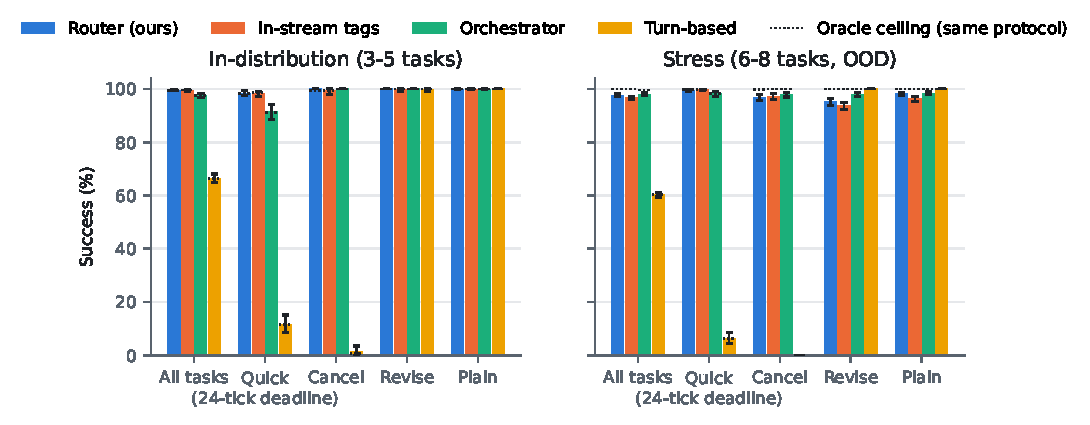
\includegraphics[width=\linewidth]{figs/success.pdf}
\caption{Success by category. Bars: mean over training seeds; error bars: 95\% bootstrap CI over 300 episodes; dotted lines: oracle ceiling for that protocol.}
\label{fig:success}
\end{figure}

\paragraph{H1, router vs.\ tags.} In distribution, the router and tags reached the same success (Table~\ref{tab:main}; $\Delta$task \dtagsidtask\,pp, CI \dtagsidtaskci; Holm-adjusted $p=\holmtagstask$). Under stress the router was more accurate ($\Delta$task \dtagsstresstask\,pp, CI \dtagsstresstaskci; $\Delta$episode \dtagsstressepisode\,pp, CI \dtagsstressepisodeci) and in both splits it generated fewer tokens ($\Delta$ \dtagsidtokens\ and \dtagsstresstokens\ tokens per episode) and answered quick tasks earlier ($\Delta$ median latency \dtagsidquicklat\ and \dtagsstressquicklat\ ticks; Table~\ref{tab:diff}). The token saving equals the channel-switch tags the tag model must spell out. Across training seeds (Table~\ref{tab:seeds}), the standard deviation of stress task success was \seedrouterstresssd\,pp for the router and \seedtagsstresssd\,pp for tags, as large as the difference, so the stress advantage should be read as tentative. H1 was supported for tokens and latency; success was equivalent in distribution and marginally higher under stress.

\paragraph{H2, router vs.\ orchestrator.} In distribution the router beat the orchestrator on quick tasks ($\Delta$ \dorchidquick\,pp, CI \dorchidquickci) and overall ($\Delta$ \dorchidtask\,pp, CI \dorchidtaskci) because the orchestrator can only react at line boundaries or by abandoning a thought. Under stress, quick-task success still favoured the router ($\Delta$ \dorchstressquick\,pp, CI \dorchstressquickci) and the router used \dorchstresstokens\ fewer tokens per episode, but overall task success did not differ ($\Delta$ \dorchstresstask\,pp, CI \dorchstresstaskci) and episode success (all tasks of an episode correct) favoured the orchestrator ($\Delta$ \dorchstressepisode\,pp, CI \dorchstressepisodeci). The orchestrator restarts abandoned thoughts from the beginning, which costs tokens but rarely leaves a half-finished line on a channel. Seed-level results (Table~\ref{tab:seeds}) agree that the two protocols are close under stress. H2 was supported for latency and quick tasks, not for overall success under stress.

\paragraph{H3, vs.\ turn-based.} The turn-based loop solved plain tasks and revisions but could not meet deadlines or honour cancellations that arrived while it was blocked (quick success \turnidquick\% in distribution, \turnstressquick\% under stress, close to its oracle ceiling of \oracleturnidquick\% and \oracleturnstressquick\%). H3 was supported by a wide margin; the size of the gap is a property of the protocol and the environment's deadlines rather than of model quality.

\begin{figure}[t]
\centering
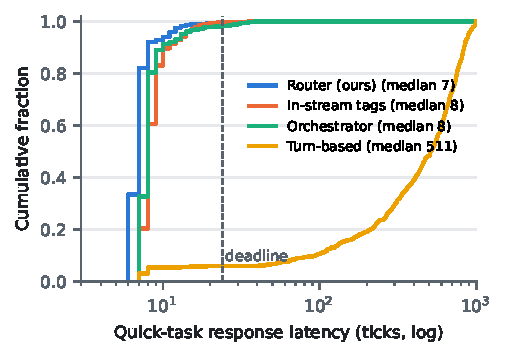
\includegraphics[width=0.55\linewidth]{figs/latency.pdf}
\caption{Quick-task response latency under stress (all seeds; unanswered tasks at the right edge).}
\label{fig:latency}
\end{figure}

\begin{table}[t]
\centering\scriptsize\setlength{\tabcolsep}{3pt}
\caption{Paired differences, router minus comparator (pp = percentage points; latency in ticks; tokens per episode). 95\% CI and two-sided bootstrap $p$ over the same 300 episodes.}
\label{tab:diff}
\resizebox{\linewidth}{!}{\begin{tabular}{llrrrrr}
\toprule
Split & Router minus & $\Delta$Task (pp) & $\Delta$Episode (pp) & $\Delta$Quick (pp) & $\Delta$Quick lat. & $\Delta$Tokens \\
\midrule
id & In-stream tags & +0.1 {\scriptsize[-0.3, +0.4]; p=0.637} & +0.5 {\scriptsize[-1.3, +2.3]; p=0.599} & -0.2 {\scriptsize[-1.5, +1.1]; p=0.844} & -1.2 {\scriptsize[-1.6, -0.8]; p=$<$0.001} & -25.1 {\scriptsize[-27.0, -23.5]; p=$<$0.001} \\
id & Orchestrator & +1.9 {\scriptsize[+1.2, +2.7]; p=$<$0.001} & +10.4 {\scriptsize[+6.7, +14.3]; p=$<$0.001} & +6.8 {\scriptsize[+4.1, +9.8]; p=$<$0.001} & -3.6 {\scriptsize[-4.3, -2.9]; p=$<$0.001} & -65.5 {\scriptsize[-70.1, -60.9]; p=$<$0.001} \\
id & Turn-based & +33.1 {\scriptsize[+31.5, +34.7]; p=$<$0.001} & +93.1 {\scriptsize[+90.3, +95.5]; p=$<$0.001} & +86.6 {\scriptsize[+83.1, +89.8]; p=$<$0.001} & -199.1 {\scriptsize[-212.5, -185.8]; p=$<$0.001} & -43.7 {\scriptsize[-47.7, -40.0]; p=$<$0.001} \\
id & Router w/o channel emb. & +0.1 {\scriptsize[-0.1, +0.2]; p=0.426} & +0.5 {\scriptsize[-0.5, +1.4]; p=0.358} & -0.2 {\scriptsize[-0.8, +0.3]; p=0.531} & +0.0 {\scriptsize[-0.1, +0.2]; p=0.555} & +0.2 {\scriptsize[-0.2, +0.6]; p=0.426} \\
stress & In-stream tags & +0.7 {\scriptsize[+0.3, +1.1]; p=0.002} & +4.9 {\scriptsize[+2.1, +7.6]; p=0.001} & +0.0 {\scriptsize[-0.4, +0.5]; p=0.910} & -1.6 {\scriptsize[-1.7, -1.4]; p=$<$0.001} & -34.4 {\scriptsize[-41.6, -26.2]; p=$<$0.001} \\
stress & Orchestrator & +0.0 {\scriptsize[-0.4, +0.4]; p=0.933} & +0.1 {\scriptsize[-2.8, +3.1]; p=0.919} & +1.4 {\scriptsize[+0.5, +2.4]; p=0.001} & -1.4 {\scriptsize[-1.7, -1.1]; p=$<$0.001} & -111.8 {\scriptsize[-122.9, -101.3]; p=$<$0.001} \\
stress & Turn-based & +37.5 {\scriptsize[+36.6, +38.4]; p=$<$0.001} & +83.7 {\scriptsize[+80.8, +86.4]; p=$<$0.001} & +93.2 {\scriptsize[+91.1, +95.2]; p=$<$0.001} & -479.8 {\scriptsize[-504.7, -453.9]; p=$<$0.001} & -144.7 {\scriptsize[-151.8, -136.5]; p=$<$0.001} \\
stress & Router w/o channel emb. & +0.3 {\scriptsize[-0.1, +0.7]; p=0.146} & +1.4 {\scriptsize[-1.1, +3.8]; p=0.258} & +0.3 {\scriptsize[-0.1, +0.7]; p=0.109} & -0.0 {\scriptsize[-0.1, +0.0]; p=0.133} & -11.8 {\scriptsize[-26.7, +1.5]; p=0.093} \\
\bottomrule
\end{tabular}
}
\end{table}

\paragraph{Ablation: channel embedding.} Removing the channel embedding, so that the model sees past tokens without their channel, did not change success ($\Delta$task \drouternoembidtask\,pp, CI \drouternoembidtaskci in distribution; Table~\ref{tab:diff}). In AsyncWorld, channel identity can apparently be inferred from content (for example the ``T$n$:'' prefix and line structure), so this ablation does not establish that the embedding is necessary.

\paragraph{H4, memory by routing.} Table~\ref{tab:long} and Figure~\ref{fig:long} report the long-horizon split (32 episodes of about 30 tasks, 1024-token cap). H4 was not supported: for the router, keeping mem-routed tokens and a plain sliding window gave the same task success ($\Delta$\,\dlongroutertask\,pp, CI \dlongroutertaskci; revisions \dlongrouterrevise\,pp, CI \dlongrouterreviseci; cancellations \dlongroutercancel\,pp, CI \dlongroutercancelci), and for tags the plain window was slightly better ($\Delta$\,\dlongtagstask\,pp, CI \dlongtagstaskci). A post-hoc stratification explains the null result: revisions and cancellations arriving more than 200 ticks after their task were solved as often as those arriving sooner under both policies (router, 99.0\% for both policies, $n=297$), so the information needed was still inside the 640-token recent window. AsyncWorld therefore did not stress retention, and with 32 episodes the test of H4 was inconclusive rather than a refutation. An unplanned finding was that \emph{not} evicting hurt: with the full, unbounded context (up to about 9k tokens, beyond the $\leq$1.2k-token training sequences) router task success fell to \longrouterfulltask\% from \longroutermemtask\%, and the model generated almost twice as many tokens (\longrouterfulltokens\ vs.\ \longroutermemtokens). We attribute this to a train/test length mismatch rather than to the method: without length generalisation or longer training sequences, an always-on model needs a bounded working context.

\begin{table}[t]
\centering\scriptsize\setlength{\tabcolsep}{3pt}
\caption{Long-horizon episodes (32 episodes, about 30 tasks over 3000 ticks) under three context policies; mean of 3 seeds with 95\% CI.}
\label{tab:long}
\resizebox{\linewidth}{!}{\begin{tabular}{llrrrrrrr}
\toprule
Arm & Eviction & Seeds & Task & Episode & Revise & Cancel & Plain & Tokens \\
\midrule
Router (ours) & none (full context) & 3 & 84.3 {\scriptsize[82.7, 86.1]} & 20.8 {\scriptsize[12.5, 31.2]} & 78.5 {\scriptsize[75.4, 82.0]} & 74.9 {\scriptsize[71.4, 78.8]} & 87.3 {\scriptsize[85.2, 89.4]} & 4578 {\scriptsize[4416, 4678]} \\
Router (ours) & keep mem-routed & 3 & 97.8 {\scriptsize[97.0, 98.5]} & 50.0 {\scriptsize[37.5, 62.5]} & 97.3 {\scriptsize[94.8, 99.2]} & 96.1 {\scriptsize[93.3, 98.4]} & 98.1 {\scriptsize[96.8, 99.1]} & 2481 {\scriptsize[2434, 2533]} \\
Router (ours) & sliding window & 3 & 97.7 {\scriptsize[97.0, 98.4]} & 49.0 {\scriptsize[36.5, 62.5]} & 97.9 {\scriptsize[95.3, 99.7]} & 96.0 {\scriptsize[93.2, 98.4]} & 98.1 {\scriptsize[97.0, 99.0]} & 2506 {\scriptsize[2451, 2562]} \\
In-stream tags & none (full context) & 3 & 91.9 {\scriptsize[89.8, 93.7]} & 14.6 {\scriptsize[7.3, 24.0]} & 93.4 {\scriptsize[90.7, 95.9]} & 95.9 {\scriptsize[92.6, 98.4]} & 90.0 {\scriptsize[87.9, 92.1]} & 2910 {\scriptsize[2648, 3257]} \\
In-stream tags & keep mem-routed & 3 & 95.0 {\scriptsize[91.8, 97.6]} & 44.8 {\scriptsize[30.2, 59.4]} & 94.6 {\scriptsize[91.0, 97.8]} & 97.3 {\scriptsize[95.1, 99.2]} & 94.2 {\scriptsize[89.8, 97.7]} & 2853 {\scriptsize[2650, 3106]} \\
In-stream tags & sliding window & 3 & 96.3 {\scriptsize[94.0, 98.1]} & 53.1 {\scriptsize[38.5, 66.7]} & 96.2 {\scriptsize[93.4, 98.4]} & 97.7 {\scriptsize[95.8, 99.3]} & 96.2 {\scriptsize[93.0, 98.4]} & 2792 {\scriptsize[2634, 3004]} \\
\bottomrule
\end{tabular}
}
\end{table}

\begin{figure}[t]
\centering
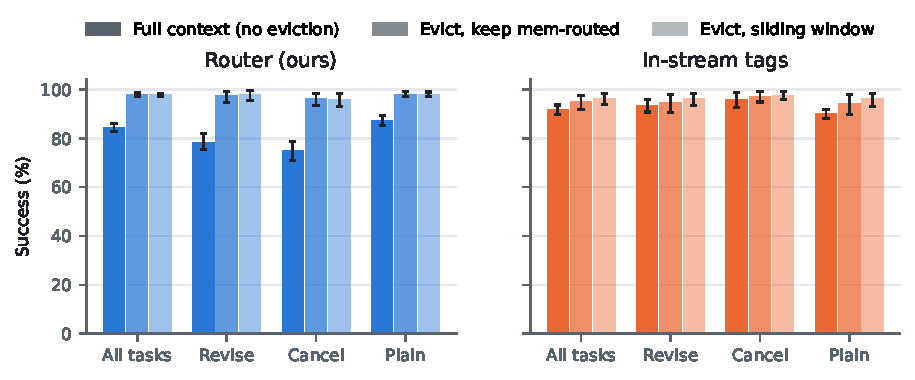
\includegraphics[width=\linewidth]{figs/long.pdf}
\caption{Long-horizon success by context policy.}
\label{fig:long}
\end{figure}

\paragraph{Multimodal pilot: seeing and reasoning in the same stream.} To test whether diverse cognitive content can share the routed stream, we trained an additional router model on a mixture of AsyncWorld episodes, visual questions and GSM8K problems \citep{cobbe2021gsm8k}. Images (synthetic scenes of 1--6 coloured circles, squares and triangles) were encoded by a frozen CLIP-ConvNeXt-Base \citep{liu2022convnext,radford2021clip} trained on LAION-2B \citep{schuhmann2022laion5b,cherti2023openclip}; the $8\times8$ feature map was pooled to 16 tokens, mapped by a trained two-layer projector \citep{liu2023llava}, and inserted on a \emph{see} channel. Visual questions asked for counts by colour or shape, existence, or the colour of a unique shape; the oracle wrote a brief think line and the answer on say. For math, we generated rationales from the base model (non-thinking mode) and kept one correct rationale per training problem (4622 of 7473), following STaR \citep{zelikman2022star} without its rationalisation step (problems with no correct sample were dropped); the rationale was routed to think and the final number to say. Training followed the two-stage recipe of LLaVA \citep{liu2023llava}: stage~1 trained only the new parameters (projector, visual position, channel embedding, router) with the LLM frozen on 30{,}000 vision-only episodes of four questions each (6.7\,M tokens); stage~2 fine-tuned all parameters on 12{,}000 mixed AsyncWorld episodes (with up to one math problem and two images each) plus 15{,}000 vision episodes with concurrent tasks (11.2\,M tokens). A first model trained with stage~2 only, on the mixed episodes alone (12{,}000 visual questions), is reported as an ablation. To check that the frozen features contained the needed information, we fitted linear probes on the 16 pooled feature vectors of the 20{,}000 training images; on the 1000 test images they predicted per-colour and per-shape object counts with 92--97\% accuracy (majority baseline 37--43\%). At test time (first 300 GSM8K test problems; 300 vision episodes with two images each on held-out scenes) we measured math accuracy with no interruptions and with two quick tasks arriving 15--120 ticks after the problem, that is, typically mid-thought, which the model must answer within the deadline before resuming. Results are in Table~\ref{tab:mm}.

\begin{table}[t]
\centering\small
\caption{Multimodal pilot (one seed per model). Accuracy in \%, bootstrap 95\% CI over items. Left: two-stage training (projector alignment, then full fine-tuning). Right: ablation trained without the alignment stage and with fewer visual examples.}
\label{tab:mm}
\begin{tabular}{lrrr}
\toprule
Evaluation & $n$ & router\_mm (two-stage) & no alignment stage \\
\midrule
GSM8K, base Qwen3-0.6B, non-thinking mode & 300 & 38.3 {\scriptsize[33.0, 43.7]} & -- \\
GSM8K, base Qwen3-0.6B, thinking mode & 300 & 53.7 {\scriptsize[48.3, 59.3]} & -- \\
GSM8K, Qwen3-0.6B, plain chat SFT on the same rationales & 300 & 52.0 {\scriptsize[46.7, 57.7]} & -- \\
GSM8K, think channel, no interruptions & 300 & 52.0 {\scriptsize[46.3, 57.7]} & 49.7 {\scriptsize[44.0, 55.0]} \\
GSM8K, 2 quick tasks arrive mid-thought & 300 & 45.7 {\scriptsize[40.0, 51.7]} & 46.3 {\scriptsize[41.0, 52.0]} \\
\quad quick tasks within deadline & 600 & 97.3 {\scriptsize[95.8, 98.5]} & 96.5 {\scriptsize[95.0, 97.8]} \\
Visual QA, all questions & 600 & 95.3 {\scriptsize[93.7, 97.0]} & 42.2 {\scriptsize[38.3, 46.3]} \\
\quad count by colour & 150 & 94.0 {\scriptsize[90.0, 97.3]} & 42.7 {\scriptsize[34.7, 50.0]} \\
\quad count by shape & 152 & 88.8 {\scriptsize[83.6, 94.1]} & 32.9 {\scriptsize[25.7, 40.8]} \\
\quad existence & 158 & 98.7 {\scriptsize[96.8, 100.0]} & 69.6 {\scriptsize[62.7, 76.6]} \\
\quad colour of unique shape & 140 & 100.0 {\scriptsize[100.0, 100.0]} & 20.7 {\scriptsize[14.3, 27.9]} \\
\quad concurrent non-visual tasks & 900 & 99.6 {\scriptsize[99.1, 99.9]} & 99.3 {\scriptsize[98.8, 99.8]} \\
AsyncWorld id episodes, all tasks & 1637 & 99.8 {\scriptsize[99.5, 99.9]} & 99.7 {\scriptsize[99.4, 99.9]} \\
\bottomrule
\end{tabular}

\end{table}

With two-stage training the single router model answered \visall\% of visual questions on held-out scenes (existence \visexists\%, colour of a unique shape \viscolorof\%, counting by colour \viscountcolor\%, counting by shape \viscountshape\%) while solving \visother\% of the concurrent non-visual tasks in the same episodes. Without the alignment stage, visual accuracy was \visallnoalign\% and the colour question was at chance (\viscolorofnoalign\% vs.\ 25\%), although the frozen features supported 92--97\% probe accuracy; the encoder was therefore not the limiting factor; because the ablation also had fewer visual examples, we cannot separate the effect of the alignment stage from that of more visual data. On GSM8K, routing self-distilled rationales to the think channel gave \gsmsolo\% without interruptions, compared with \gsmbase\% for the base model in non-thinking mode\gsmthinkclause; the router did not differ from thinking mode (paired $\Delta$\,\gsmvsthink\,pp, CI \gsmvsthinkci) while using a median of \gsmthinktok\ think tokens per problem. When two quick tasks arrived during the thought, the model answered \gsmasyncquick\% of them within the deadline and resumed, but math accuracy fell to \gsmasync\% (paired difference \gsmdiff\,pp, CI \gsmdiffci; $n=300$). Pausing and resuming a train of thought therefore had a measurable cost at this scale. AsyncWorld performance remained high with the added modalities (\mmidtask\% task success in distribution; text-only router \routeridtask\%, different seeds and task mixture).

\section{Discussion}
The results support a narrow claim: in a controlled environment, a small LLM can learn to select its own output channel token by token, to wait without terminating, and to handle interruptions at their arrival time, with no external controller and with task success close to its scripted teacher in distribution. A learned router head was as accurate as spelling channel tags into the text and avoided their token overhead. Relative to a rule-based orchestrator, in-model control mainly bought latency and tokens; overall success under heavy load was similar. The largest effect, against a turn-based loop, follows from what that protocol can express. The multimodal pilot showed that a visual sense and multi-step reasoning can be added to the same routed stream without degrading the agentic behaviour, provided the visual features are first aligned; it also exposed a cost of interrupting reasoning that a brain-like system would need to manage. The memory channel did not help in our environment, which leaves its value open.

\paragraph{What the analogy suggests next.} The brain analogy points to experiments we did not run: (i) more senses (audio frames inserted on a hear channel at their arrival time; video as a sequence of image events); (ii) learned rather than scripted policies, by reinforcement learning on environment reward, since imitation caps performance at the oracle; (iii) richer think content (planning, hypothesis testing, critique) from stronger teachers; (iv) parallel effectors, for example speaking while writing, which a single stream can only interleave; (v) consolidation, in which mem-routed content is written to weights or an external store.

\section{Limitations}
\begin{itemize}\itemsep0pt
\item \textbf{Synthetic tasks and imitation.} AsyncWorld is small and scripted; all arms imitate scripted oracles; models came within about a point of their oracle ceilings on task success in distribution, but under stress the router's episode success was \routerstressepisode\% against an oracle ceiling of \oraclerouterstressepisode\%; differences between arms partly reflect the design of each protocol's oracle rather than learned strategies.
\item \textbf{Scale.} One 0.6B model, one epoch, three to five seeds per arm; the multimodal model has one seed. Effects may differ at scale.
\item \textbf{Missing baselines.} We did not compare against published agent systems \citep{li2026never} on their benchmarks, did not ablate idle against EOS, and did not train a matched plain-SFT model on the same GSM8K rationales.
\item \textbf{Baselines.} The orchestrator and turn-based arms are our implementations of these control styles, trained on the same data; they are not the published systems \citep{li2026never,yao2022react}.
\item \textbf{Oracle corrections.} During the study we found that the oracle could suspend a say line for a quick answer on the same channel, which merged two lines in about 12\% of router and tags episodes. We fixed the oracle, rebuilt the data and retrained all affected arms; superseded checkpoints and runs were archived. A related resume-order error in the multimodal oracle was fixed before that model was trained.
\item \textbf{Interrupted reasoning.} Suspending a math rationale for urgent requests reduced GSM8K accuracy by \gsmdiff\,pp; the oracle resumes the thought verbatim, and the model may need explicit training to re-establish context after a pause.
\item \textbf{Memory.} AsyncWorld rarely required information older than the recent window, so the mem-retention hypothesis was not tested in a regime where it could matter; the retention budget and window were fixed, not tuned; long-horizon results rest on 32 episodes.
\item \textbf{Brain analogy.} The mapping in Table~\ref{tab:brain} is a design heuristic. We did not compare model activity with neural data.
\end{itemize}

\section{Ethics and broader impact}
All data were synthetic or public (GSM8K, MIT licence \citep{cobbe2021gsm8k}); no human participants or personal data were involved. An always-on model that acts without an external controller moves safety-relevant decisions (when to call a tool, when to act) into learned weights; deployments would still need external permission checks and sandboxing of tool execution, which this design does not replace.

\section{Conclusion}
Replacing the stop token with a learned idle action, routing every token to an output channel with a small head, and inserting events at their true arrival time let a single LLM think, speak, write, code, call tools, remember and wait without an agent loop. In controlled synthetic tests this matched in-stream tags with fewer tokens, answered urgent requests faster than a rule-based orchestrator at similar overall success, and, as expected by construction, handled interrupts far better than a turn-based loop. The multimodal pilot shows that vision and step-by-step reasoning can share the same routed stream. Whether the approach helps on natural, open-ended tasks remains to be tested.

\paragraph{Reproducibility.} Environment, oracle, data builder, training, rollout and analysis code, the hypotheses document, all test-episode seeds and per-episode result files are available at \url{https://github.com/SiavashShirzad/NeverIdleMind}.

\bibliographystyle{plainnat}
\bibliography{refs}

\appendix
\section{Example trace}\label{app:trace}
Table~\ref{tab:trace} shows the first in-distribution test episode for router seed~0, as generated in closed loop. Consecutive tokens with the same source and channel are merged; $\hookleftarrow$ marks a newline, which completes a line on that channel. Inputs are inserted wherever they arrive: the cancellation of T2 interrupts a thought, the requests for T4 and T5 arrive in the middle of think lines, and the quick task T6 arrives in the middle of a mem line, which the model suspends, answers on say, and then completes.
\begin{table}[h]
\centering\scriptsize
\caption{Closed-loop trace (router, seed 0, test episode 0).}
\label{tab:trace}
\begin{tabular}{llp{11.5cm}}
\toprule
Source & Channel & Tokens \\
\midrule
\textbf{model} & \texttt{idle} & \texttt{\textless{}|idle|\textgreater{}} \\
\textit{input} & \texttt{user} & \texttt{T1 quick: 9+5? $\hookleftarrow$} \\
\textbf{model} & \texttt{say} & \texttt{T1: 14 $\hookleftarrow$} \\
\textbf{model} & \texttt{idle} & \texttt{\textless{}|idle|\textgreater{}} \\
\textit{input} & \texttt{user} & \texttt{T2 ask: what is the code for kiwi? $\hookleftarrow$} \\
\textbf{model} & \texttt{think} & \texttt{T2 needs the code for kiwi. That needs the lookup tool; I will report it when the} \\
\textit{input} & \texttt{user} & \texttt{cancel T2 $\hookleftarrow$} \\
\textbf{model} & \texttt{think} & \texttt{The user cancelled T2} \\
\textit{input} & \texttt{user} & \texttt{T3 ask: what is (83+81)*18? $\hookleftarrow$} \\
\textbf{model} & \texttt{think} & \texttt{. I drop it and will ignore any result for it. $\hookleftarrow$} \\
\textbf{model} & \texttt{mem} & \texttt{T2 cancelled $\hookleftarrow$} \\
\textbf{model} & \texttt{think} & \texttt{T3} \\
\textit{input} & \texttt{user} & \texttt{T4 code: count multiples of 7 below 17 $\hookleftarrow$} \\
\textbf{model} & \texttt{think} & \texttt{wants (} \\
\textit{input} & \texttt{user} & \texttt{T5 write: sort 49 91 87 73 54 $\hookleftarrow$} \\
\textbf{model} & \texttt{think} & \texttt{83+81)*18. I should not do this in my head, so I will call calc and wait for the result. $\hookleftarrow$} \\
\textbf{model} & \texttt{mem} & \texttt{T3 open calc (} \\
\textit{input} & \texttt{user} & \texttt{T6 quick: 1+3? $\hookleftarrow$} \\
\textbf{model} & \texttt{say} & \texttt{T6: 4 $\hookleftarrow$} \\
\textbf{model} & \texttt{mem} & \texttt{83+81)*18 $\hookleftarrow$} \\
\textbf{model} & \texttt{exec} & \texttt{T3 calc (83+81)*18 $\hookleftarrow$} \\
\textbf{model} & \texttt{think} & \texttt{T4 needs the count multiples of 7 below 17. I will write one line of python, run it, and say the output. $\hookleftarrow$} \\
\textbf{model} & \texttt{mem} & \texttt{T4 open code $\hookleftarrow$} \\
\textbf{model} & \texttt{code} & \texttt{T4: print(len([i for i in range(1} \\
\textit{input} & \texttt{tool} & \texttt{T3 calc (83+81)*18 = 2952 $\hookleftarrow$} \\
\textbf{model} & \texttt{code} & \texttt{,17) if i\%7==0])) $\hookleftarrow$} \\
\textbf{model} & \texttt{exec} & \texttt{T4 run $\hookleftarrow$} \\
\textbf{model} & \texttt{say} & \texttt{T3: 2952 $\hookleftarrow$} \\
\textbf{model} & \texttt{mem} & \texttt{T3 closed $\hookleftarrow$} \\
\textbf{model} & \texttt{think} & \texttt{T5 is a sorting job for 49 91 87 73 5} \\
\textit{input} & \texttt{tool} & \texttt{T4 output: 2 $\hookleftarrow$} \\
\textbf{model} & \texttt{think} & \texttt{4. No tool needed; put them in increasing order and write them down. $\hookleftarrow$} \\
\textbf{model} & \texttt{write} & \texttt{T5: 49 54 73 87 91 $\hookleftarrow$} \\
\textbf{model} & \texttt{mem} & \texttt{T5 closed $\hookleftarrow$} \\
\textbf{model} & \texttt{say} & \texttt{T4: 2 $\hookleftarrow$} \\
\textbf{model} & \texttt{mem} & \texttt{T4 closed $\hookleftarrow$} \\
\textbf{model} & \texttt{idle} & \texttt{\textless{}|idle|\textgreater{}} \\
\bottomrule
\end{tabular}

\end{table}

\section{Seed-level results}\label{app:seeds}
\begin{table}[h]
\centering\small
\caption{Task success per training seed and across seeds (mean, SD and $t$-based 95\% CI over seeds).}
\label{tab:seeds}
\resizebox{\linewidth}{!}{\begin{tabular}{llrlrr}
\toprule
Split & Arm & Seeds & Task success per seed (\%) & Mean $\pm$ SD & 95\% CI (seeds, $t$) \\
\midrule
id & Router (ours) & 3 & 99.4, 99.5, 99.7 & 99.6 $\pm$ 0.2 & [99.2, 99.9] \\
id & In-stream tags & 3 & 99.3, 99.5, 99.5 & 99.4 $\pm$ 0.1 & [99.1, 99.7] \\
id & Orchestrator & 3 & 97.7, 97.5, 97.6 & 97.6 $\pm$ 0.1 & [97.3, 97.9] \\
id & Turn-based & 3 & 66.4, 66.5, 66.5 & 66.5 $\pm$ 0.0 & [66.4, 66.5] \\
id & Router w/o channel emb. & 3 & 99.2, 99.6, 99.6 & 99.5 $\pm$ 0.3 & [98.8, 100.1] \\
stress & Router (ours) & 3 & 98.6, 96.7, 97.8 & 97.7 $\pm$ 0.9 & [95.4, 100.0] \\
stress & In-stream tags & 3 & 98.4, 95.5, 96.3 & 96.8 $\pm$ 1.5 & [93.1, 100.4] \\
stress & Orchestrator & 3 & 97.5, 98.1, 98.5 & 98.0 $\pm$ 0.5 & [96.7, 99.4] \\
stress & Turn-based & 3 & 60.3, 60.3, 60.3 & 60.3 $\pm$ 0.0 & [60.3, 60.3] \\
stress & Router w/o channel emb. & 3 & 97.2, 97.6, 97.7 & 97.5 $\pm$ 0.3 & [96.8, 98.2] \\
\bottomrule
\end{tabular}
}
\end{table}

\section{Training details}\label{app:train}
\begin{table}[h]
\centering\small
\caption{Training and evaluation settings (identical for all arms unless noted).}
\begin{tabular}{ll}
\toprule
Base model & Qwen3-0.6B, full fine-tuning, tied embeddings \\
New parameters & channel embedding (zero init), router $\mathrm{Linear}(1024,7)$; tag tokens for tag arms \\
Optimiser & AdamW, $\beta=(0.9,0.95)$, no weight decay, lr $5\times10^{-5}$ (new parameters $10^{-3}$) \\
Schedule & 30-step warm-up, cosine decay, 1 epoch \\
Batch & length-bucketed, 16{,}384 tokens (multimodal: 12{,}288) \\
Precision & fp32 master weights, bf16 autocast, gradient checkpointing \\
Training data & 12{,}000 id episodes + 600 long episodes $\times$ 4 eviction views; 7.4--8.3\,M tokens per arm \\
Context & cap 1024 tokens; recent window 640; mem budget 192 \\
Decoding & greedy; step cap 3000 (9000 for long episodes) \\
Hardware & one NVIDIA RTX 4090 per run; about 13\,min per training run \\
\bottomrule
\end{tabular}
\end{table}
\end{document}
